\documentclass[1p]{elsarticle_modified}
%\bibliographystyle{elsarticle-num}

%\usepackage[colorlinks]{hyperref}
%\usepackage{abbrmath_seonhwa} %\Abb, \Ascr, \Acal ,\Abf, \Afrak
\usepackage{amsfonts}
\usepackage{amssymb}
\usepackage{amsmath}
\usepackage{amsthm}
\usepackage{scalefnt}
\usepackage{amsbsy}
\usepackage{kotex}
\usepackage{caption}
\usepackage{subfig}
\usepackage{color}
\usepackage{graphicx}
\usepackage{xcolor} %% white, black, red, green, blue, cyan, magenta, yellow
\usepackage{float}
\usepackage{setspace}
\usepackage{hyperref}

\usepackage{tikz}
\usetikzlibrary{arrows}

\usepackage{multirow}
\usepackage{array} % fixed length table
\usepackage{hhline}

%%%%%%%%%%%%%%%%%%%%%
\makeatletter
\renewcommand*\env@matrix[1][\arraystretch]{%
	\edef\arraystretch{#1}%
	\hskip -\arraycolsep
	\let\@ifnextchar\new@ifnextchar
	\array{*\c@MaxMatrixCols c}}
\makeatother %https://tex.stackexchange.com/questions/14071/how-can-i-increase-the-line-spacing-in-a-matrix
%%%%%%%%%%%%%%%

\usepackage[normalem]{ulem}

\newcommand{\msout}[1]{\ifmmode\text{\sout{\ensuremath{#1}}}\else\sout{#1}\fi}
%SOURCE: \msout is \stkout macro in https://tex.stackexchange.com/questions/20609/strikeout-in-math-mode

\newcommand{\cancel}[1]{
	\ifmmode
	{\color{red}\msout{#1}}
	\else
	{\color{red}\sout{#1}}
	\fi
}

\newcommand{\add}[1]{
	{\color{blue}\uwave{#1}}
}

\newcommand{\replace}[2]{
	\ifmmode
	{\color{red}\msout{#1}}{\color{blue}\uwave{#2}}
	\else
	{\color{red}\sout{#1}}{\color{blue}\uwave{#2}}
	\fi
}

\newcommand{\Sol}{\mathcal{S}} %segment
\newcommand{\D}{D} %diagram
\newcommand{\A}{\mathcal{A}} %arc


%%%%%%%%%%%%%%%%%%%%%%%%%%%%%5 test

\def\sl{\operatorname{\textup{SL}}(2,\Cbb)}
\def\psl{\operatorname{\textup{PSL}}(2,\Cbb)}
\def\quan{\mkern 1mu \triangleright \mkern 1mu}

\theoremstyle{definition}
\newtheorem{thm}{Theorem}[section]
\newtheorem{prop}[thm]{Proposition}
\newtheorem{lem}[thm]{Lemma}
\newtheorem{ques}[thm]{Question}
\newtheorem{cor}[thm]{Corollary}
\newtheorem{defn}[thm]{Definition}
\newtheorem{exam}[thm]{Example}
\newtheorem{rmk}[thm]{Remark}
\newtheorem{alg}[thm]{Algorithm}

\newcommand{\I}{\sqrt{-1}}
\begin{document}

%\begin{frontmatter}
%
%\title{Boundary parabolic representations of knots up to 8 crossings}
%
%%% Group authors per affiliation:
%\author{Yunhi Cho} 
%\address{Department of Mathematics, University of Seoul, Seoul, Korea}
%\ead{yhcho@uos.ac.kr}
%
%
%\author{Seonhwa Kim} %\fnref{s_kim}}
%\address{Center for Geometry and Physics, Institute for Basic Science, Pohang, 37673, Korea}
%\ead{ryeona17@ibs.re.kr}
%
%\author{Hyuk Kim}
%\address{Department of Mathematical Sciences, Seoul National University, Seoul 08826, Korea}
%\ead{hyukkim@snu.ac.kr}
%
%\author{Seokbeom Yoon}
%\address{Department of Mathematical Sciences, Seoul National University, Seoul, 08826,  Korea}
%\ead{sbyoon15@snu.ac.kr}
%
%\begin{abstract}
%We find all boundary parabolic representation of knots up to 8 crossings.
%
%\end{abstract}
%\begin{keyword}
%    \MSC[2010] 57M25 
%\end{keyword}
%
%\end{frontmatter}

%\linenumbers
%\tableofcontents
%
\newcommand\colored[1]{\textcolor{white}{\rule[-0.35ex]{0.8em}{1.4ex}}\kern-0.8em\color{red} #1}%
%\newcommand\colored[1]{\textcolor{white}{ #1}\kern-2.17ex	\textcolor{white}{ #1}\kern-1.81ex	\textcolor{white}{ #1}\kern-2.15ex\color{red}#1	}

{\Large $\underline{10_{55}~(K10a_{9})}$}

\setlength{\tabcolsep}{10pt}
\renewcommand{\arraystretch}{1.6}
\vspace{1cm}\begin{tabular}{m{100pt}>{\centering\arraybackslash}m{274pt}}
\multirow{5}{120pt}{
	\centering
	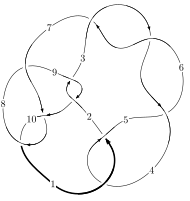
\includegraphics[width=112pt]{../../../GIT/diagram.site/Diagrams/png/139_10_55.png}\\
\ \ \ A knot diagram\footnotemark}&
\allowdisplaybreaks
\textbf{Linearized knot diagam} \\
\cline{2-2}
 &
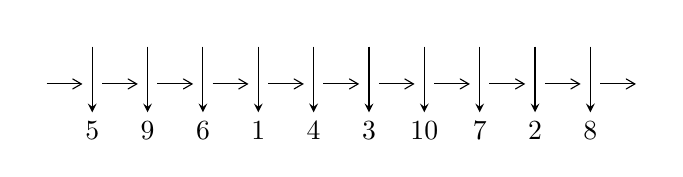
\begin{tikzpicture}[x=20pt, y=17pt]
	% nodes
	\node (C0) at (0, 0) {};
	\node (C1) at (1, 0) {};
	\node (C1U) at (1, +1) {};
	\node (C1D) at (1, -1) {5};

	\node (C2) at (2, 0) {};
	\node (C2U) at (2, +1) {};
	\node (C2D) at (2, -1) {9};

	\node (C3) at (3, 0) {};
	\node (C3U) at (3, +1) {};
	\node (C3D) at (3, -1) {6};

	\node (C4) at (4, 0) {};
	\node (C4U) at (4, +1) {};
	\node (C4D) at (4, -1) {1};

	\node (C5) at (5, 0) {};
	\node (C5U) at (5, +1) {};
	\node (C5D) at (5, -1) {4};

	\node (C6) at (6, 0) {};
	\node (C6U) at (6, +1) {};
	\node (C6D) at (6, -1) {3};

	\node (C7) at (7, 0) {};
	\node (C7U) at (7, +1) {};
	\node (C7D) at (7, -1) {10};

	\node (C8) at (8, 0) {};
	\node (C8U) at (8, +1) {};
	\node (C8D) at (8, -1) {7};

	\node (C9) at (9, 0) {};
	\node (C9U) at (9, +1) {};
	\node (C9D) at (9, -1) {2};

	\node (C10) at (10, 0) {};
	\node (C10U) at (10, +1) {};
	\node (C10D) at (10, -1) {8};
	\node (C11) at (11, 0) {};

	% arrows
	\draw[->,>={angle 60}]
	(C0) edge (C1) (C1) edge (C2) (C2) edge (C3) (C3) edge (C4) (C4) edge (C5) (C5) edge (C6) (C6) edge (C7) (C7) edge (C8) (C8) edge (C9) (C9) edge (C10) (C10) edge (C11) ;	\draw[->,>=stealth]
	(C1U) edge (C1D) (C2U) edge (C2D) (C3U) edge (C3D) (C4U) edge (C4D) (C5U) edge (C5D) (C6U) edge (C6D) (C7U) edge (C7D) (C8U) edge (C8D) (C9U) edge (C9D) (C10U) edge (C10D) ;
	\end{tikzpicture} \\
\hhline{~~} \\& 
\textbf{Solving Sequence} \\ \cline{2-2} 
 &
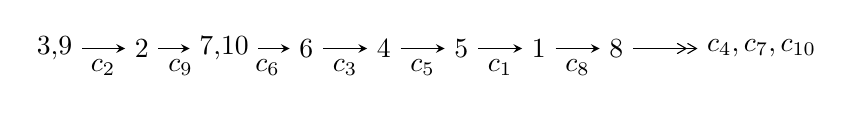
\begin{tikzpicture}[x=28pt, y=7pt]
	% node
	\node (A0) at (-1/8, 0) {3,9};
	\node (A1) at (1, 0) {2};
	\node (A2) at (33/16, 0) {7,10};
	\node (A3) at (25/8, 0) {6};
	\node (A4) at (33/8, 0) {4};
	\node (A5) at (41/8, 0) {5};
	\node (A6) at (49/8, 0) {1};
	\node (A7) at (57/8, 0) {8};
	\node (C1) at (1/2, -1) {$c_{2}$};
	\node (C2) at (3/2, -1) {$c_{9}$};
	\node (C3) at (21/8, -1) {$c_{6}$};
	\node (C4) at (29/8, -1) {$c_{3}$};
	\node (C5) at (37/8, -1) {$c_{5}$};
	\node (C6) at (45/8, -1) {$c_{1}$};
	\node (C7) at (53/8, -1) {$c_{8}$};
	\node (A8) at (9, 0) {$c_{4},c_{7},c_{10}$};

	% edge
	\draw[->,>=stealth]	
	(A0) edge (A1) (A1) edge (A2) (A2) edge (A3) (A3) edge (A4) (A4) edge (A5) (A5) edge (A6) (A6) edge (A7) ;
	\draw[->>,>={angle 60}]	
	(A7) edge (A8);
\end{tikzpicture} \\ 

\end{tabular} \\

\footnotetext{
The image of knot diagram is generated by the software ``\textbf{Draw programme}" developed by Andrew Bartholomew(\url{http://www.layer8.co.uk/maths/draw/index.htm\#Running-draw}), where we modified some parts for our purpose(\url{https://github.com/CATsTAILs/LinksPainter}).
}\phantom \\ \newline 
\centering \textbf{Ideals for irreducible components\footnotemark of $X_{\text{par}}$} 
 
\begin{align*}
I^u_{1}&=\langle 
-6.12530\times10^{24} u^{32}+1.02963\times10^{25} u^{31}+\cdots+2.34036\times10^{25} b+4.69152\times10^{25},\\
\phantom{I^u_{1}}&\phantom{= \langle  }-1.57092\times10^{25} u^{32}+3.30476\times10^{25} u^{31}+\cdots+9.36144\times10^{25} a+1.45111\times10^{26},\;u^{33}- u^{32}+\cdots+12 u+8\rangle \\
\\
I^v_{1}&=\langle 
a,\;- v^2+b-2 v-1,\;v^3+2 v^2+v+1\rangle \\
\end{align*}
\raggedright * 2 irreducible components of $\dim_{\mathbb{C}}=0$, with total 36 representations.\\
\footnotetext{All coefficients of polynomials are rational numbers. But the coefficients are sometimes approximated in decimal forms when there is not enough margin.}
\newpage
\renewcommand{\arraystretch}{1}
\centering \section*{I. $I^u_{1}= \langle -6.13\times10^{24} u^{32}+1.03\times10^{25} u^{31}+\cdots+2.34\times10^{25} b+4.69\times10^{25},\;-1.57\times10^{25} u^{32}+3.30\times10^{25} u^{31}+\cdots+9.36\times10^{25} a+1.45\times10^{26},\;u^{33}- u^{32}+\cdots+12 u+8 \rangle$}
\flushleft \textbf{(i) Arc colorings}\\
\begin{tabular}{m{7pt} m{180pt} m{7pt} m{180pt} }
\flushright $a_{3}=$&$\begin{pmatrix}1\\0\end{pmatrix}$ \\
\flushright $a_{9}=$&$\begin{pmatrix}0\\u\end{pmatrix}$ \\
\flushright $a_{2}=$&$\begin{pmatrix}1\\- u^2\end{pmatrix}$ \\
\flushright $a_{7}=$&$\begin{pmatrix}0.167808 u^{32}-0.353018 u^{31}+\cdots-2.39523 u-1.55009\\0.261725 u^{32}-0.439945 u^{31}+\cdots+2.01891 u-2.00462\end{pmatrix}$ \\
\flushright $a_{10}=$&$\begin{pmatrix}- u\\u^3+u\end{pmatrix}$ \\
\flushright $a_{6}=$&$\begin{pmatrix}0.429532 u^{32}-0.792963 u^{31}+\cdots-0.376322 u-3.55471\\0.261725 u^{32}-0.439945 u^{31}+\cdots+2.01891 u-2.00462\end{pmatrix}$ \\
\flushright $a_{4}=$&$\begin{pmatrix}0.334706 u^{32}-0.0742812 u^{31}+\cdots+3.75000 u+2.50288\\0.0757738 u^{32}-0.0652588 u^{31}+\cdots-4.16452 u-1.47047\end{pmatrix}$ \\
\flushright $a_{5}=$&$\begin{pmatrix}0.0320196 u^{32}+0.277867 u^{31}+\cdots+5.92497 u+1.20624\\-0.211499 u^{32}+0.571258 u^{31}+\cdots+6.09759 u+3.97229\end{pmatrix}$ \\
\flushright $a_{1}=$&$\begin{pmatrix}-0.429532 u^{32}+0.792963 u^{31}+\cdots+0.376322 u+3.55471\\-0.0675857 u^{32}+0.312561 u^{31}+\cdots+2.94382 u+0.902830\end{pmatrix}$ \\
\flushright $a_{8}=$&$\begin{pmatrix}0.309620 u^{32}-0.669262 u^{31}+\cdots-2.20116 u-2.87870\\0.249910 u^{32}-0.483907 u^{31}+\cdots+0.866167 u-2.07146\end{pmatrix}$\\&\end{tabular}
\flushleft \textbf{(ii) Obstruction class $= -1$}\\~\\
\flushleft \textbf{(iii) Cusp Shapes $= -\frac{60635423650415331489185849}{46807175136350804609973980} u^{32}+\frac{108124405345856702791639919}{46807175136350804609973980} u^{31}+\cdots+\frac{483007911642190145433442939}{23403587568175402304986990} u+\frac{98098888352311967905148621}{11701793784087701152493495}$}\\~\\
\newpage\renewcommand{\arraystretch}{1}
\flushleft \textbf{(iv) u-Polynomials at the component}\newline \\
\begin{tabular}{m{50pt}|m{274pt}}
Crossings & \hspace{64pt}u-Polynomials at each crossing \\
\hline $$\begin{aligned}c_{1},c_{4}\end{aligned}$$&$\begin{aligned}
&u^{33}+2 u^{32}+\cdots+3 u+1
\end{aligned}$\\
\hline $$\begin{aligned}c_{2},c_{9}\end{aligned}$$&$\begin{aligned}
&u^{33}- u^{32}+\cdots+12 u+8
\end{aligned}$\\
\hline $$\begin{aligned}c_{3},c_{5},c_{6}\end{aligned}$$&$\begin{aligned}
&u^{33}+8 u^{32}+\cdots+11 u+1
\end{aligned}$\\
\hline $$\begin{aligned}c_{7},c_{10}\end{aligned}$$&$\begin{aligned}
&u^{33}-4 u^{32}+\cdots-16 u^2+1
\end{aligned}$\\
\hline $$\begin{aligned}c_{8}\end{aligned}$$&$\begin{aligned}
&u^{33}+14 u^{32}+\cdots+32 u+1
\end{aligned}$\\
\hline
\end{tabular}\\~\\
\newpage\renewcommand{\arraystretch}{1}
\flushleft \textbf{(v) Riley Polynomials at the component}\newline \\
\begin{tabular}{m{50pt}|m{274pt}}
Crossings & \hspace{64pt}Riley Polynomials at each crossing \\
\hline $$\begin{aligned}c_{1},c_{4}\end{aligned}$$&$\begin{aligned}
&y^{33}-8 y^{32}+\cdots+11 y-1
\end{aligned}$\\
\hline $$\begin{aligned}c_{2},c_{9}\end{aligned}$$&$\begin{aligned}
&y^{33}+21 y^{32}+\cdots-304 y-64
\end{aligned}$\\
\hline $$\begin{aligned}c_{3},c_{5},c_{6}\end{aligned}$$&$\begin{aligned}
&y^{33}+36 y^{32}+\cdots-29 y-1
\end{aligned}$\\
\hline $$\begin{aligned}c_{7},c_{10}\end{aligned}$$&$\begin{aligned}
&y^{33}-14 y^{32}+\cdots+32 y-1
\end{aligned}$\\
\hline $$\begin{aligned}c_{8}\end{aligned}$$&$\begin{aligned}
&y^{33}+14 y^{32}+\cdots+340 y-1
\end{aligned}$\\
\hline
\end{tabular}\\~\\
\newpage\flushleft \textbf{(vi) Complex Volumes and Cusp Shapes}
$$\begin{array}{c|c|c}  
\text{Solutions to }I^u_{1}& \I (\text{vol} + \sqrt{-1}CS) & \text{Cusp shape}\\
 \hline 
\begin{aligned}
u &= \phantom{-}0.287842 + 0.978115 I \\
a &= \phantom{-}0.995506 - 0.250345 I \\
b &= -0.990032 + 0.166252 I\end{aligned}
 & -1.68836 - 2.02472 I & -12.19123 + 3.15987 I \\ \hline\begin{aligned}
u &= \phantom{-}0.287842 - 0.978115 I \\
a &= \phantom{-}0.995506 + 0.250345 I \\
b &= -0.990032 - 0.166252 I\end{aligned}
 & -1.68836 + 2.02472 I & -12.19123 - 3.15987 I \\ \hline\begin{aligned}
u &= -0.258728 + 1.015690 I \\
a &= \phantom{-}0.614647 + 0.062246 I \\
b &= -0.555531 + 0.902494 I\end{aligned}
 & \phantom{-}1.90081 + 2.94788 I & -6.37142 - 4.00779 I \\ \hline\begin{aligned}
u &= -0.258728 - 1.015690 I \\
a &= \phantom{-}0.614647 - 0.062246 I \\
b &= -0.555531 - 0.902494 I\end{aligned}
 & \phantom{-}1.90081 - 2.94788 I & -6.37142 + 4.00779 I \\ \hline\begin{aligned}
u &= \phantom{-}0.044652 + 1.064410 I \\
a &= \phantom{-}0.01862 - 1.72371 I \\
b &= -0.12788 - 1.49913 I\end{aligned}
 & \phantom{-}3.40289 - 3.09457 I & -6.42907 + 2.76186 I \\ \hline\begin{aligned}
u &= \phantom{-}0.044652 - 1.064410 I \\
a &= \phantom{-}0.01862 + 1.72371 I \\
b &= -0.12788 + 1.49913 I\end{aligned}
 & \phantom{-}3.40289 + 3.09457 I & -6.42907 - 2.76186 I \\ \hline\begin{aligned}
u &= \phantom{-}0.818675 + 0.392192 I \\
a &= \phantom{-}0.407864 - 1.122020 I \\
b &= -0.568824 + 0.589839 I\end{aligned}
 & -2.18443 + 2.93057 I & -13.2700 - 5.9877 I \\ \hline\begin{aligned}
u &= \phantom{-}0.818675 - 0.392192 I \\
a &= \phantom{-}0.407864 + 1.122020 I \\
b &= -0.568824 - 0.589839 I\end{aligned}
 & -2.18443 - 2.93057 I & -13.2700 + 5.9877 I \\ \hline\begin{aligned}
u &= -1.163260 + 0.173959 I \\
a &= -0.077899 - 0.940641 I \\
b &= -0.05060 + 1.49956 I\end{aligned}
 & \phantom{-}5.10374 + 0.60080 I & -6.85884 + 0.13509 I \\ \hline\begin{aligned}
u &= -1.163260 - 0.173959 I \\
a &= -0.077899 + 0.940641 I \\
b &= -0.05060 - 1.49956 I\end{aligned}
 & \phantom{-}5.10374 - 0.60080 I & -6.85884 - 0.13509 I\\
 \hline 
 \end{array}$$\newpage$$\begin{array}{c|c|c}  
\text{Solutions to }I^u_{1}& \I (\text{vol} + \sqrt{-1}CS) & \text{Cusp shape}\\
 \hline 
\begin{aligned}
u &= \phantom{-}0.004841 + 1.181600 I \\
a &= -0.834891 - 0.002237 I \\
b &= \phantom{-}0.261591 + 0.605055 I\end{aligned}
 & \phantom{-}3.34637 + 1.37148 I & -3.58776 - 2.92200 I \\ \hline\begin{aligned}
u &= \phantom{-}0.004841 - 1.181600 I \\
a &= -0.834891 + 0.002237 I \\
b &= \phantom{-}0.261591 - 0.605055 I\end{aligned}
 & \phantom{-}3.34637 - 1.37148 I & -3.58776 + 2.92200 I \\ \hline\begin{aligned}
u &= \phantom{-}1.169540 + 0.246902 I \\
a &= \phantom{-}0.090452 - 0.991567 I \\
b &= -0.17482 + 1.55316 I\end{aligned}
 & \phantom{-}4.94269 + 5.66526 I & -7.31949 - 5.14166 I \\ \hline\begin{aligned}
u &= \phantom{-}1.169540 - 0.246902 I \\
a &= \phantom{-}0.090452 + 0.991567 I \\
b &= -0.17482 - 1.55316 I\end{aligned}
 & \phantom{-}4.94269 - 5.66526 I & -7.31949 + 5.14166 I \\ \hline\begin{aligned}
u &= -0.360189 + 1.214590 I \\
a &= -1.071120 - 0.076444 I \\
b &= \phantom{-}0.414527 - 0.386927 I\end{aligned}
 & \phantom{-}2.58252 + 3.89244 I & -4.89744 - 3.42674 I \\ \hline\begin{aligned}
u &= -0.360189 - 1.214590 I \\
a &= -1.071120 + 0.076444 I \\
b &= \phantom{-}0.414527 + 0.386927 I\end{aligned}
 & \phantom{-}2.58252 - 3.89244 I & -4.89744 + 3.42674 I \\ \hline\begin{aligned}
u &= \phantom{-}0.513708 + 1.159100 I \\
a &= \phantom{-}1.164090 - 0.112067 I \\
b &= -0.819767 - 0.833430 I\end{aligned}
 & \phantom{-}0.26767 - 7.94172 I & -10.29455 + 8.51301 I \\ \hline\begin{aligned}
u &= \phantom{-}0.513708 - 1.159100 I \\
a &= \phantom{-}1.164090 + 0.112067 I \\
b &= -0.819767 + 0.833430 I\end{aligned}
 & \phantom{-}0.26767 + 7.94172 I & -10.29455 - 8.51301 I \\ \hline\begin{aligned}
u &= \phantom{-}0.354082 + 0.631353 I \\
a &= \phantom{-}0.44471 - 1.78764 I \\
b &= -0.534495 - 0.382584 I\end{aligned}
 & -2.82990 - 0.89439 I & -12.3753 + 7.1209 I \\ \hline\begin{aligned}
u &= \phantom{-}0.354082 - 0.631353 I \\
a &= \phantom{-}0.44471 + 1.78764 I \\
b &= -0.534495 + 0.382584 I\end{aligned}
 & -2.82990 + 0.89439 I & -12.3753 - 7.1209 I\\
 \hline 
 \end{array}$$\newpage$$\begin{array}{c|c|c}  
\text{Solutions to }I^u_{1}& \I (\text{vol} + \sqrt{-1}CS) & \text{Cusp shape}\\
 \hline 
\begin{aligned}
u &= -0.659340 + 0.056414 I \\
a &= -0.636628 - 0.442458 I \\
b &= -0.073834 + 0.218596 I\end{aligned}
 & -0.946260 - 0.088153 I & -9.34082 - 0.77609 I \\ \hline\begin{aligned}
u &= -0.659340 - 0.056414 I \\
a &= -0.636628 + 0.442458 I \\
b &= -0.073834 - 0.218596 I\end{aligned}
 & -0.946260 + 0.088153 I & -9.34082 + 0.77609 I \\ \hline\begin{aligned}
u &= \phantom{-}0.000493 + 0.636688 I \\
a &= \phantom{-}0.198636 - 0.514130 I \\
b &= -0.289339 + 1.220180 I\end{aligned}
 & \phantom{-}2.22875 + 2.67528 I & -2.73278 - 2.26366 I \\ \hline\begin{aligned}
u &= \phantom{-}0.000493 - 0.636688 I \\
a &= \phantom{-}0.198636 + 0.514130 I \\
b &= -0.289339 - 1.220180 I\end{aligned}
 & \phantom{-}2.22875 - 2.67528 I & -2.73278 + 2.26366 I \\ \hline\begin{aligned}
u &= -0.40839 + 1.41713 I \\
a &= \phantom{-}0.780933 + 0.268916 I \\
b &= -0.19663 + 1.64569 I\end{aligned}
 & \phantom{-}10.43260 + 6.00927 I & -4.11461 - 3.31809 I \\ \hline\begin{aligned}
u &= -0.40839 - 1.41713 I \\
a &= \phantom{-}0.780933 - 0.268916 I \\
b &= -0.19663 - 1.64569 I\end{aligned}
 & \phantom{-}10.43260 - 6.00927 I & -4.11461 + 3.31809 I \\ \hline\begin{aligned}
u &= \phantom{-}0.34967 + 1.43738 I \\
a &= -0.805445 + 0.250021 I \\
b &= \phantom{-}0.04143 + 1.56263 I\end{aligned}
 & \phantom{-}10.72190 + 0.46043 I & -3.63720 - 1.59605 I \\ \hline\begin{aligned}
u &= \phantom{-}0.34967 - 1.43738 I \\
a &= -0.805445 - 0.250021 I \\
b &= \phantom{-}0.04143 - 1.56263 I\end{aligned}
 & \phantom{-}10.72190 - 0.46043 I & -3.63720 + 1.59605 I \\ \hline\begin{aligned}
u &= \phantom{-}0.64547 + 1.35144 I \\
a &= \phantom{-}1.222060 - 0.008698 I \\
b &= -0.27678 - 1.65105 I\end{aligned}
 & \phantom{-}8.4689 - 12.1855 I & -6.56707 + 7.63472 I \\ \hline\begin{aligned}
u &= \phantom{-}0.64547 - 1.35144 I \\
a &= \phantom{-}1.222060 + 0.008698 I \\
b &= -0.27678 + 1.65105 I\end{aligned}
 & \phantom{-}8.4689 + 12.1855 I & -6.56707 - 7.63472 I\\
 \hline 
 \end{array}$$\newpage$$\begin{array}{c|c|c}  
\text{Solutions to }I^u_{1}& \I (\text{vol} + \sqrt{-1}CS) & \text{Cusp shape}\\
 \hline 
\begin{aligned}
u &= -0.60403 + 1.37429 I \\
a &= -1.203410 + 0.000498 I \\
b &= \phantom{-}0.11865 - 1.50838 I\end{aligned}
 & \phantom{-}8.95423 + 5.75725 I & -5.65390 - 2.88970 I \\ \hline\begin{aligned}
u &= -0.60403 - 1.37429 I \\
a &= -1.203410 - 0.000498 I \\
b &= \phantom{-}0.11865 + 1.50838 I\end{aligned}
 & \phantom{-}8.95423 - 5.75725 I & -5.65390 + 2.88970 I \\ \hline\begin{aligned}
u &= -0.470095\phantom{ +0.000000I} \\
a &= -0.116243\phantom{ +0.000000I} \\
b &= -0.355337\phantom{ +0.000000I}\end{aligned}
 & -0.842528\phantom{ +0.000000I} & -11.7170\phantom{ +0.000000I}\\
 \hline 
 \end{array}$$\newpage\newpage\renewcommand{\arraystretch}{1}
\centering \section*{II. $I^v_{1}= \langle a,\;- v^2+b-2 v-1,\;v^3+2 v^2+v+1 \rangle$}
\flushleft \textbf{(i) Arc colorings}\\
\begin{tabular}{m{7pt} m{180pt} m{7pt} m{180pt} }
\flushright $a_{3}=$&$\begin{pmatrix}1\\0\end{pmatrix}$ \\
\flushright $a_{9}=$&$\begin{pmatrix}v\\0\end{pmatrix}$ \\
\flushright $a_{2}=$&$\begin{pmatrix}1\\0\end{pmatrix}$ \\
\flushright $a_{7}=$&$\begin{pmatrix}0\\v^2+2 v+1\end{pmatrix}$ \\
\flushright $a_{10}=$&$\begin{pmatrix}v\\0\end{pmatrix}$ \\
\flushright $a_{6}=$&$\begin{pmatrix}v^2+2 v+1\\v^2+2 v+1\end{pmatrix}$ \\
\flushright $a_{4}=$&$\begin{pmatrix}v^2+v\\v^2+v-1\end{pmatrix}$ \\
\flushright $a_{5}=$&$\begin{pmatrix}v^2+v\\- v-1\end{pmatrix}$ \\
\flushright $a_{1}=$&$\begin{pmatrix}0\\- v^2-2 v-1\end{pmatrix}$ \\
\flushright $a_{8}=$&$\begin{pmatrix}v\\v^2+2 v+1\end{pmatrix}$\\&\end{tabular}
\flushleft \textbf{(ii) Obstruction class $= 1$}\\~\\
\flushleft \textbf{(iii) Cusp Shapes $= 2 v^2+5 v-11$}\\~\\
\newpage\renewcommand{\arraystretch}{1}
\flushleft \textbf{(iv) u-Polynomials at the component}\newline \\
\begin{tabular}{m{50pt}|m{274pt}}
Crossings & \hspace{64pt}u-Polynomials at each crossing \\
\hline $$\begin{aligned}c_{1}\end{aligned}$$&$\begin{aligned}
&u^3+u^2-1
\end{aligned}$\\
\hline $$\begin{aligned}c_{2},c_{9}\end{aligned}$$&$\begin{aligned}
&u^3
\end{aligned}$\\
\hline $$\begin{aligned}c_{3}\end{aligned}$$&$\begin{aligned}
&u^3- u^2+2 u-1
\end{aligned}$\\
\hline $$\begin{aligned}c_{4}\end{aligned}$$&$\begin{aligned}
&u^3- u^2+1
\end{aligned}$\\
\hline $$\begin{aligned}c_{5},c_{6}\end{aligned}$$&$\begin{aligned}
&u^3+u^2+2 u+1
\end{aligned}$\\
\hline $$\begin{aligned}c_{7}\end{aligned}$$&$\begin{aligned}
&(u-1)^3
\end{aligned}$\\
\hline $$\begin{aligned}c_{8},c_{10}\end{aligned}$$&$\begin{aligned}
&(u+1)^3
\end{aligned}$\\
\hline
\end{tabular}\\~\\
\newpage\renewcommand{\arraystretch}{1}
\flushleft \textbf{(v) Riley Polynomials at the component}\newline \\
\begin{tabular}{m{50pt}|m{274pt}}
Crossings & \hspace{64pt}Riley Polynomials at each crossing \\
\hline $$\begin{aligned}c_{1},c_{4}\end{aligned}$$&$\begin{aligned}
&y^3- y^2+2 y-1
\end{aligned}$\\
\hline $$\begin{aligned}c_{2},c_{9}\end{aligned}$$&$\begin{aligned}
&y^3
\end{aligned}$\\
\hline $$\begin{aligned}c_{3},c_{5},c_{6}\end{aligned}$$&$\begin{aligned}
&y^3+3 y^2+2 y-1
\end{aligned}$\\
\hline $$\begin{aligned}c_{7},c_{8},c_{10}\end{aligned}$$&$\begin{aligned}
&(y-1)^3
\end{aligned}$\\
\hline
\end{tabular}\\~\\
\newpage\flushleft \textbf{(vi) Complex Volumes and Cusp Shapes}
$$\begin{array}{c|c|c}  
\text{Solutions to }I^v_{1}& \I (\text{vol} + \sqrt{-1}CS) & \text{Cusp shape}\\
 \hline 
\begin{aligned}
v &= -0.122561 + 0.744862 I \\
a &= \phantom{-0.000000 } 0 \\
b &= \phantom{-}0.215080 + 1.307140 I\end{aligned}
 & \phantom{-}1.37919 - 2.82812 I & -12.69240 + 3.35914 I \\ \hline\begin{aligned}
v &= -0.122561 - 0.744862 I \\
a &= \phantom{-0.000000 } 0 \\
b &= \phantom{-}0.215080 - 1.307140 I\end{aligned}
 & \phantom{-}1.37919 + 2.82812 I & -12.69240 - 3.35914 I \\ \hline\begin{aligned}
v &= -1.75488\phantom{ +0.000000I} \\
a &= \phantom{-0.000000 } 0 \\
b &= \phantom{-}0.569840\phantom{ +0.000000I}\end{aligned}
 & -2.75839\phantom{ +0.000000I} & -13.6150\phantom{ +0.000000I}\\
 \hline 
 \end{array}$$\newpage
\newpage\renewcommand{\arraystretch}{1}
\centering \section*{ III. u-Polynomials}
\begin{tabular}{m{50pt}|m{274pt}}
Crossings & \hspace{64pt}u-Polynomials at each crossing \\
\hline $$\begin{aligned}c_{1}\end{aligned}$$&$\begin{aligned}
&(u^3+u^2-1)(u^{33}+2 u^{32}+\cdots+3 u+1)
\end{aligned}$\\
\hline $$\begin{aligned}c_{2},c_{9}\end{aligned}$$&$\begin{aligned}
&u^3(u^{33}- u^{32}+\cdots+12 u+8)
\end{aligned}$\\
\hline $$\begin{aligned}c_{3}\end{aligned}$$&$\begin{aligned}
&(u^3- u^2+2 u-1)(u^{33}+8 u^{32}+\cdots+11 u+1)
\end{aligned}$\\
\hline $$\begin{aligned}c_{4}\end{aligned}$$&$\begin{aligned}
&(u^3- u^2+1)(u^{33}+2 u^{32}+\cdots+3 u+1)
\end{aligned}$\\
\hline $$\begin{aligned}c_{5},c_{6}\end{aligned}$$&$\begin{aligned}
&(u^3+u^2+2 u+1)(u^{33}+8 u^{32}+\cdots+11 u+1)
\end{aligned}$\\
\hline $$\begin{aligned}c_{7}\end{aligned}$$&$\begin{aligned}
&((u-1)^3)(u^{33}-4 u^{32}+\cdots-16 u^2+1)
\end{aligned}$\\
\hline $$\begin{aligned}c_{8}\end{aligned}$$&$\begin{aligned}
&((u+1)^3)(u^{33}+14 u^{32}+\cdots+32 u+1)
\end{aligned}$\\
\hline $$\begin{aligned}c_{10}\end{aligned}$$&$\begin{aligned}
&((u+1)^3)(u^{33}-4 u^{32}+\cdots-16 u^2+1)
\end{aligned}$\\
\hline
\end{tabular}\newpage\renewcommand{\arraystretch}{1}
\centering \section*{ IV. Riley Polynomials}
\begin{tabular}{m{50pt}|m{274pt}}
Crossings & \hspace{64pt}Riley Polynomials at each crossing \\
\hline $$\begin{aligned}c_{1},c_{4}\end{aligned}$$&$\begin{aligned}
&(y^3- y^2+2 y-1)(y^{33}-8 y^{32}+\cdots+11 y-1)
\end{aligned}$\\
\hline $$\begin{aligned}c_{2},c_{9}\end{aligned}$$&$\begin{aligned}
&y^3(y^{33}+21 y^{32}+\cdots-304 y-64)
\end{aligned}$\\
\hline $$\begin{aligned}c_{3},c_{5},c_{6}\end{aligned}$$&$\begin{aligned}
&(y^3+3 y^2+2 y-1)(y^{33}+36 y^{32}+\cdots-29 y-1)
\end{aligned}$\\
\hline $$\begin{aligned}c_{7},c_{10}\end{aligned}$$&$\begin{aligned}
&((y-1)^3)(y^{33}-14 y^{32}+\cdots+32 y-1)
\end{aligned}$\\
\hline $$\begin{aligned}c_{8}\end{aligned}$$&$\begin{aligned}
&((y-1)^3)(y^{33}+14 y^{32}+\cdots+340 y-1)
\end{aligned}$\\
\hline
\end{tabular}
\vskip 2pc
\end{document}